\begin{frame}{}
    \LARGE Diffusion Models: \textbf{Noise Schedules}
\end{frame}


\begin{frame}{Noise Schedules}
    \begin{columns}
    \begin{column}{0.45\textwidth}
       \begin{itemize}
            \item The noise schedule $\{\beta_t\}$ controls the amount of noise added at each timestep.
            \item<2-> Common schedules:
            \begin{itemize}
                \item \textbf{Linear:} Simple and intuitive.
                \item \textbf{Cosine:} Preserves perceptual signal longer; often yields better image generation results.
            \end{itemize}
            \item<3-> The choice of schedule impacts training dynamics and the quality of generated samples.
            \item<4-> Visualizing different schedules helps understand how noise accumulates over time.
        \end{itemize}
    \end{column}
    \begin{column}{0.55\textwidth}
        \begin{figure}
            \centering
            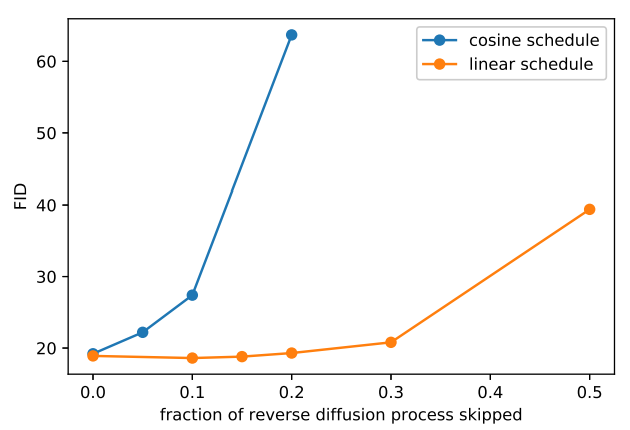
\includegraphics[height=\textheight, width=\textwidth, keepaspectratio]{images/diffusion/noise_schedules.png}
            \caption*{Comparison of linear and cosine noise schedules.}
        \end{figure}
    \end{column}
\end{columns}
\end{frame}